% -*- TeX -*- -*- UK -*- -*- Soft -*-

\chapter{Mathematical Intuition behind Gradient Descent}
\label{sec:MathematicalIntuitionbehindGradientDescent}


Mathematical derivation of the update rule in Gradient Descent---the most popular optimization algorithm in Machine Learning and Deep Learning.

Shahbaz Khan


\lstinline{https://towardsdatascience.com/mathematical-intuition-behind-gradient-descent-f1b959a59e6d} 

\section{Introduction}

If you've ever seen or heard of the term 'Gradient Descent' in your life, you must have most certainly come across the following equation for gradient descent parameter update:
\begin{marginfigure}
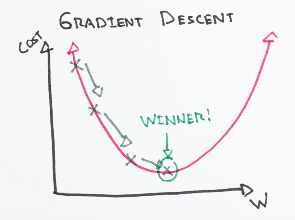
\includegraphics{graddescent01}
\end{marginfigure}
\begin{equation}
\theta_{n e w}=\theta-\alpha * \frac{\delta L}{\delta \theta}
\end{equation}

In the above equation $L$ is a loss function (or a cost function) and $\theta$ is any parameter on which the cost function depends. These are weights ($W$) and biases ($b$) in case of Neural Networks (or Deep Learning).

The goal is to find the global minima of the loss function.
These parameters are updated during each iteration of training algorithm until we reach a minimum value of the loss function.

In the context of Deep Learning (or Neural Networks), we write the above equations in terms of weights and biases, as:

\begin{equation}
\begin{array}{c}{w_{n e w}=w-\alpha * \frac{\delta L}{\delta w}} \\ {b_{n e w}=b-\alpha * \frac{\delta L}{\delta b}}\end{array}
\end{equation}
This is a fundamental step in Gradient Descent optimization algorithm, that is executed during each iteration of training.

Let's derive this equation mathematically (don't panic ! all you need is high school basic calculus to do this). After doing this, whenever you encounter the parameter update step you would know of its origins, and feel more empowered !

\section{General Learning Algorithm}

Let's first quickly review the general Learning Algorithm:
\begin{marginfigure}
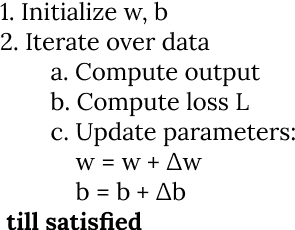
\includegraphics{graddescent02}
\end{marginfigure}

Here 'till satisfied' is a subjective condition and could be one of the many stopping criteria such as reaching threshold loss value or iterating some fixed number of times, etc.

\section{Parameter Update Step}

Note that the update step involves adding  some change $\Delta  w$, $\Delta  b$ to $w$,$b$. We will soon find out that those are indeed negative partial derivatives of loss w.r.t $w$,$b$ respectively i.e $-\delta \mathbf{L} / \delta w$ and $-\delta \mathbf{L} / \delta b$ where $L = f(w,b)$.

Let us formulate these mathematically:
\begin{equation}
\begin{array}{c}{\text { Let } \theta=[w, b]} \\ {\Delta \theta=[\Delta w, \Delta b]} \\ {\theta_{\text {new}}=\theta+\Delta \theta}\end{array}
\end{equation}
We need a principled approach to find $\Delta \theta$ so that $L\left(\theta_{n e w}\right)<L(\theta)$.
Note that we have not introduced learning rate $\alpha$  yet. Let's first understand the need of learning rates.

\section{Need for Learning Rate}

We know that $\theta$ is a vector, and so is $\Delta  \theta$.

Let us consider the sum of these two vectors
\begin{marginfigure}
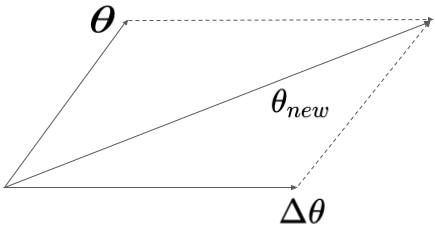
\includegraphics{graddescent03}
\end{marginfigure}



It is evident that the resultant sum of the two vectors is quite large compared to individual vectors. This is because we are taking a large step $\Delta  \theta$. We need to take small steps in that direction so that vector sum is small. This is also important because if we make such large updates ($\Delta  \theta$) to parameters $\theta$, we might miss out on global minimum of loss function L. Hence we introduce learning rate $\alpha$  that limits the size of update we make to parameters $\theta$. Observe the vector sum of $\theta$ and $\alpha \Delta  \theta$
\begin{marginfigure}
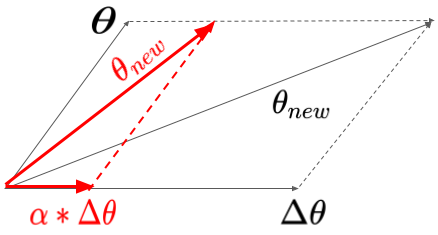
\includegraphics{graddescent04}
\end{marginfigure}



Note how, with the help of learning rate $\alpha  < 1$, we limit the amount of update we make to $\theta$.

Let us now find out the correct value of $\Delta  \theta$ that will reduce the value of loss.

Before we move ahead, let me introduce the (in)famous Taylor Series, which we will use to find $\Delta  w$, $\Delta  b$ and hence $\Delta  \theta$.

\section{Taylor Series and its application in Gradient Descent}
\begin{equation}
f(x+\Delta x)=f(x)+f^{\prime}(x) \Delta x+\frac{1}{2 !} f^{\prime \prime}(x) \Delta x^{2}+\frac{1}{3 !} f^{\prime \prime \prime}(x) \Delta x^{3}+\ldots
\end{equation}

Taylor's series is used to find the value of a function at a distance $\Delta  x$ from a point $x$, given the derivatives of the function at that point.

Let's find the value of $\Delta  w$ using Taylor's series.
In this case, function $f$ will be loss function $L$, and we will expand the series for $L(w + \alpha *\Delta  w)$.

We have to find a value of $\Delta  w$ such that $L(w + \alpha *\Delta  w) < L(w)$.
\begin{equation}
L(w+\alpha \Delta w)=L(w)+\alpha L^{\prime}(w) \Delta x+\frac{\alpha^{2}}{2 !} L^{\prime \prime}(w) \Delta w^{2}+\frac{\alpha^{3}}{3 !} L^{\prime \prime \prime}(w) \Delta w^{3}+\ldots
\end{equation}
At this step, we can infer that we'd need second term onwards to be negative for the new loss to be smaller than the old loss.

But Loss $L(\theta)$ is a multivariate function. It is a function of not just weight $w$, but also bias $b$. We have represented them as a vector $\theta = [w, b]$.

So we need to write down the vector form of Taylor series to find $\Delta  \theta$.
\begin{equation}
L(\theta+\alpha \Delta \theta)=L(\theta)+\alpha \Delta \theta^{T} \nabla_{\theta} L(\theta)+\frac{\alpha^{2}}{2 !} \Delta \theta^{T} \nabla_{\theta}^{2} L(\theta)+\frac{\alpha^{3}}{3 !} \Delta \theta^{T} \nabla_{\theta}^{3} L(\theta)+\ldots
\end{equation}


Here $\nabla  L(\theta)$ represents first-order gradient of loss w.r.t $\theta$.
Gradient is nothing but a vector of partial derivatives of the function w.r.t each of its parameters.

Similarly $\nabla^2$ will be a vector of second-order partial derivatives and so on.

In practice learning rate $\alpha$  is very small (0.001, 0.00001, etc.), so $\alpha^2$, $\alpha^3$, etc. will be very small and their contribution to the loss $L$ will be negligible.
So they can be ignored from the equation.
The final equation will then become
\begin{equation}
L(\theta+\alpha \Delta \theta) \approx L(\theta)+\alpha \Delta \theta^{T} \nabla_{\theta} L(\theta)
\end{equation}


\section{Finding best value for $\Delta  \theta$}

Since we want the updated loss $L(\theta + \alpha \Delta  \theta)$ to be less than the previous loss $L(\theta)$, and since loss is a positive quantity, the second term in above equation has to be negative.
So we need such value of $\Delta  \theta$ so that the dot product in second term becomes negative, i.e we need 
\begin{equation}
\Delta \theta^{T} \nabla_{\theta} L(\theta)<0
\end{equation}
Let's consider the angle between $\Delta \theta$ and $\nabla_\theta$
\begin{marginfigure}
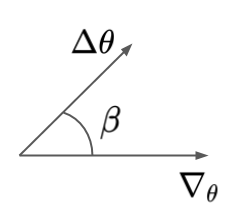
\includegraphics{graddescent05}
\end{marginfigure}




We know that the cosine of angle between 2 vectors is their dot product divided by product of their magnitudes
\begin{equation}
\cos \beta=\frac{\Delta \theta^{T} \nabla_{\theta}}{|\Delta \theta|\left|\nabla_{\theta}\right|}
\end{equation}

We also know that $\cos\beta$ lies between $-1$ and $1$ i.e $-1 \leq\cos\beta \leq +1 $.
Therefore,
\begin{equation}
-1 \leq \cos \beta=\frac{\Delta \theta^{T} \nabla_{\theta}}{|\Delta \theta|\left|\nabla_{\theta}\right|} \leq+1
\end{equation}
Let's multiple throughout by $\mathrm{k}=|\Delta \theta|\left|\nabla_{\theta}\right|$
\begin{equation}
-k \leq \Delta \theta^{T} \nabla_{\theta} \leq+k
\end{equation}



Now we want the dot product to be as negative as possible (so that loss can be as low as possible)
But as we can see from the above inequality, the most negative value it can acquire is $-k$.

Now for the dot product to be $-k$, $\cos\beta$ has to be equal to -1.
$\cos\beta=-1$, which  corresponds to $\beta = 180^\circ$
\begin{marginfigure}
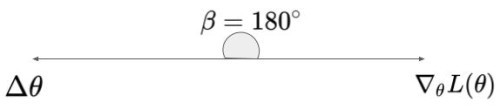
\includegraphics{graddescent06}
\end{marginfigure}


Since the two vectors are in opposite direction, from vector properties we know
\begin{equation}
\Delta \theta=-\nabla_{\theta} L(\theta)
\end{equation}
i.e.,
\begin{equation}
\left[\begin{array}{l}{\Delta w} \\ {\Delta b}\end{array}\right]=-\left[\begin{array}{c}{\frac{\delta L}{\delta w}} \\ {\frac{\delta L}{\delta b}}\end{array}\right]
\end{equation}




\section{Final Parameter Update Step}

Now if we substitute these values in the parameter update step in general learning algorithm, it becomes
\begin{equation}
\begin{aligned} w &=w-\alpha * \frac{\delta L}{\delta w} \\ b &=b-\alpha * \frac{\delta L}{\delta b} \end{aligned}
\end{equation}

Now that equation is similar to what we set out to derive.
Each time you update your parameters ($w$ and $b$) using this rule, the loss on your training set will decrease, until it cannot reduce further i.e when slopes(or partial derivatives) become 0. The result in decrease of loss due to iterative update steps is shown in the figure.


\begin{marginfigure}
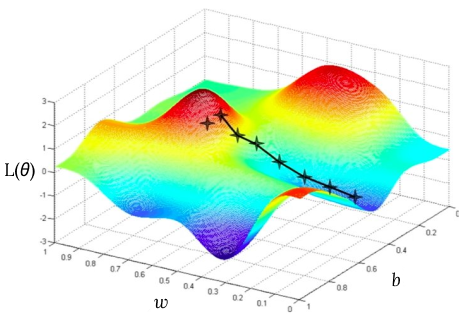
\includegraphics{graddescent07}
\end{marginfigure}

\section{Gradient Descent Rule for multiple weights and biases}

We have derived the update rule for a single weight and bias.
In reality a deep neural network has a lot of weights and biases, which are represented as matrices (or tensors), and so our update rule should also be modified to update all weights and biases of the network simultaneously.

    Note that most deep learning texts use the notation $\Delta$   instead of $\nabla$  to represent gradient in equations.

\begin{equation}
\begin{array}{l}{\mathrm{W}=\mathrm{W}-\alpha \Delta W} \\ {\mathrm{b}=\mathrm{b}-\alpha \Delta b}\end{array}
\end{equation}

\begin{equation}
W=\left[
\begin{array}{cccc}
w_{11}& w_{12}& \ldots& w_{1 n}\\ 
w_{21}& w_{22}& \ldots& w_{2 n} \\ 
&\vdots \\ 
w_{n 1}& w_{n 2} &\ldots &w_{n n}
\end{array}
\right]
\end{equation}

\begin{equation}
\Delta W=
\left[
\begin{array}{cccc}
{\frac{\delta L}{\delta w_{11}}} & {\frac{\delta L}{\delta w_{12}}} & {\dots} & {\frac{\delta L}{\delta w_{1 n}}} \\ 
{\frac{\delta L}{\delta w_{21}}} & {\frac{\delta L}{\delta w_{22}}} & {\cdots} & {\frac{\delta L}{\delta w_{2 n}}} \\ 
{} & {\vdots} \\ 
{\frac{\delta L}{\delta w_{n 1}}} &{\frac{\delta L}{\delta w_{n 2}}} & {\cdots} & {\frac{\delta L}{\delta w_{n n}}}
\end{array}
\right]
\end{equation}

\section{Conclusion}

That is all for this one. I hope after reading this, you have developed a more intuitive understanding of gradient descent algorithm. 